\documentclass{article} % Oder eine andere Dokumentklasse wie report, book, etc.
\usepackage[utf8]{inputenc} % Bestimmt die Eingabe-Kodierung
\usepackage[T1]{fontenc} % Bestimmt die Ausgabe-Kodierung
\usepackage{graphicx}


\begin{document}
	
	\title{Deep Reinforcement Learning Exercise 05}
	\maketitle
	
	Group:
	\begin{itemize}
		\item Marvin Kohnen
		\item Moritz Gehring
		\item Julius Ferber 
		
	\end{itemize}
	\section{Exercise 5.1}
	
	\subsection{5.1a}
	We implemented the algorithm as intended.
	Figure \ref{fig:1} shows the Average Episode Rewards over 100 Episodes, while Figure \ref{fig:2} shows the same regarding the Loss. Both graphs show spikes at the same episodes. 
	Some episodes resulted in high average rewards, suggesting that at particular times the agent was effective at maximizing rewards during its interactions with the environment (successful balancing of the cart in CartPole). Similarly, the graph for average episode loss also shows substantial spikes. High fluctuations in loss indicate inconstencies in how well the Q values are being approximated relative to the target values. These spikes suggest, that the agent is still not entirely stable and is likely still exploring. Furthermore, the inherent instability of DQN is certainly contributing to the behaviour of the agent. 
	
	\textit{Reflection}:
	In order to visualize the value function, we could fix the velocity of the cart and the angular velocity of the pole, and then plot the value function for the remaining two variables, namely the position of the cart and the angle of the pole.
	This could help us understand the value function better, and how it changes when the cart moves or the pole tilts, where critical points are or where the value function is unstable.
	
	\begin{figure}[h!]
		\centering
		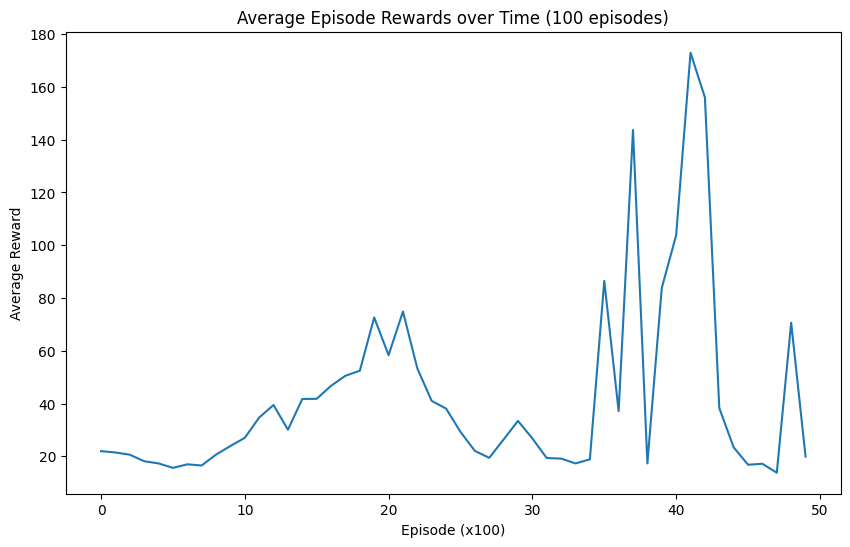
\includegraphics[width=0.9\textwidth]{images/1a_1.png}
		\caption{Average Episode Rewards over Time (100 Episodes)}
		\label{fig:1}
	\end{figure}
	
	\begin{figure}[h!]
		\centering
		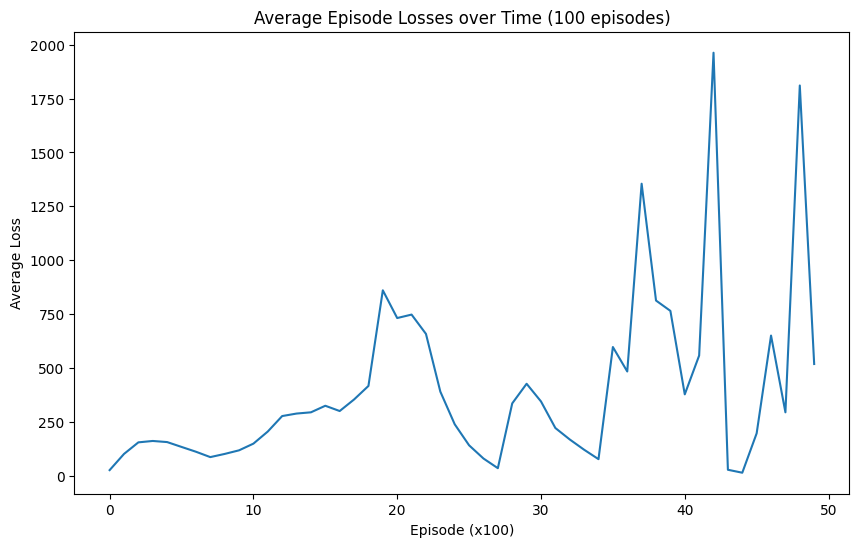
\includegraphics[width=0.9\textwidth]{images/1a_2.png}
		\caption{Average Episode Losses over Time (100 Episodes)}
		\label{fig:2}
	\end{figure}
	
	\newpage
	
	\subsection{5.1b}
	We implemented a replay buffer. The blue line in Figure \ref{fig:3} top (indicating the average rewards) shows a significant increase over time, reaching up to around 500. This increase reflects the agent's ability to learn an effective policy that balances the pole correctly and maximizes rewards consistently throughout episodes.
	The rewards curve is generally smoother than before, which suggests that the replay buffer helps stabilize the learning process by injecting diverse experiences into the training, leading to consistent improvement. The difference in height to the agent without replay buffer also indicates an overall better performance when a replay buffer is implemented.
	
	As the replay buffer allows the model to accumulate more steps per episode, the accumulated loss naturally rises (see Figure \ref{fig:3} bottom, blue line). Similarly to the reward structure, the average Episode losses also look quite stable.
	
	
	Figure \ref{fig:4} shows the value function and policy with regards to Pole Angle over Cart Position without a replay buffer implemented. The policy heatmap indicates a less refined action selection across the state space. The agent likely doesn't have sufficient experience to choose the optimal actions, leading to poor performance overall.
	The distribution appears to be biased towards certain states, particularly at various angles, suggesting that the model's understanding of the environment is limited.
	
	In contrast, Figure \ref{fig:5} displays the same graphs, but with an implemented replay buffer. The policy heatmap shows a more comprehensive understanding of action selection. The agent effectively learns to select actions based on the pole's angle and cart position, achieving a more balanced response that accounts for a wider range of states.
	The stronger gradient in policy indicates refined action choices and a better overall understanding of the environment, yielding better control. This improvement may explain the better performance displayed in Figure \ref{fig:3}.
	
	
	\begin{figure}[h!]
		\centering
		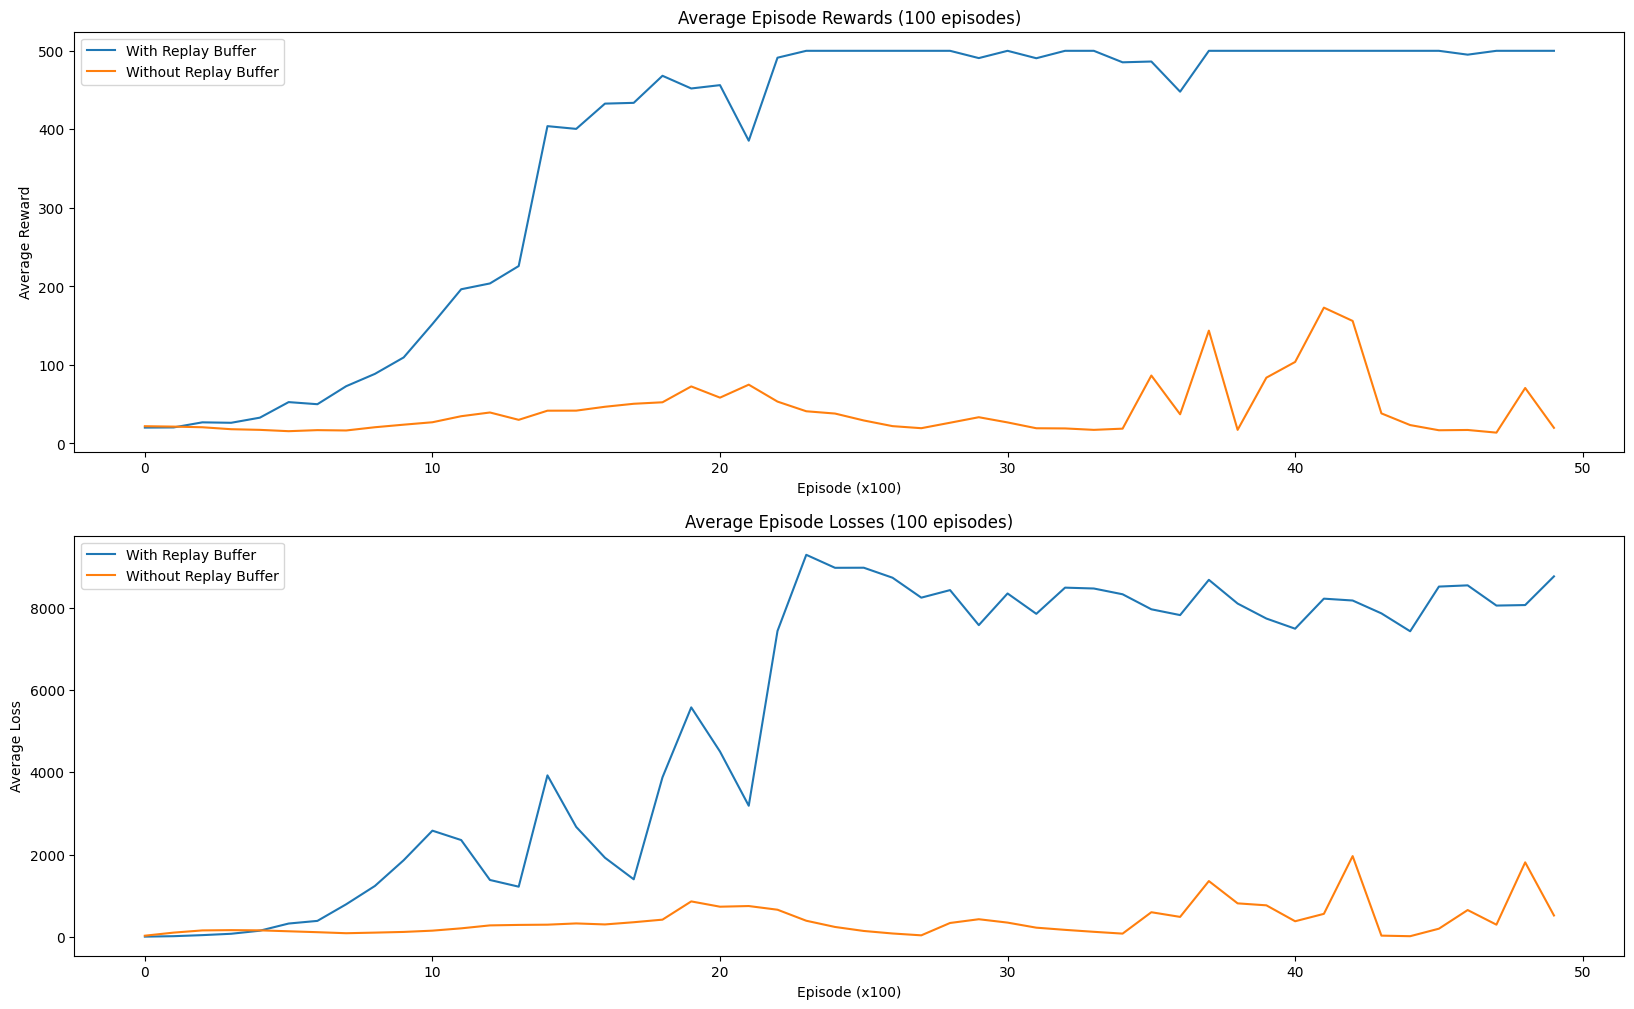
\includegraphics[width=0.9\textwidth]{images/1b_1.png}
		\caption{Average Episode Rewards and Losses over Time (100 Episodes)}
		\label{fig:3}
	\end{figure}
	
	
	\begin{figure}[h!]
		\centering
		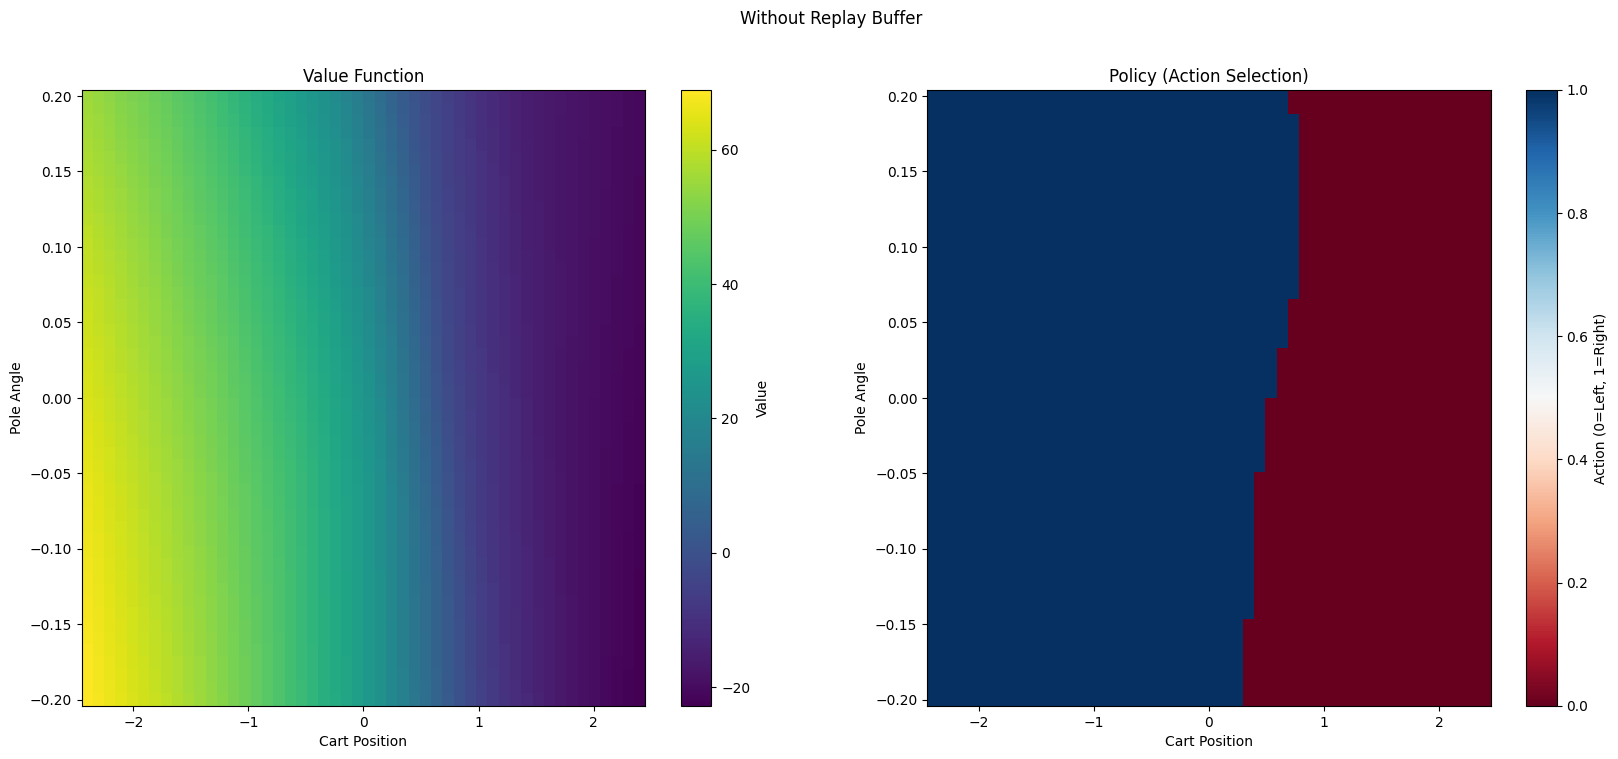
\includegraphics[width=0.9\textwidth]{images/1b_2.png}
		\caption{Value function and Policy with regrads to Pole Angle over Cart Position without Replay Buffer}
		\label{fig:4}
	\end{figure}
	
	
	\begin{figure}[h!]
		\centering
		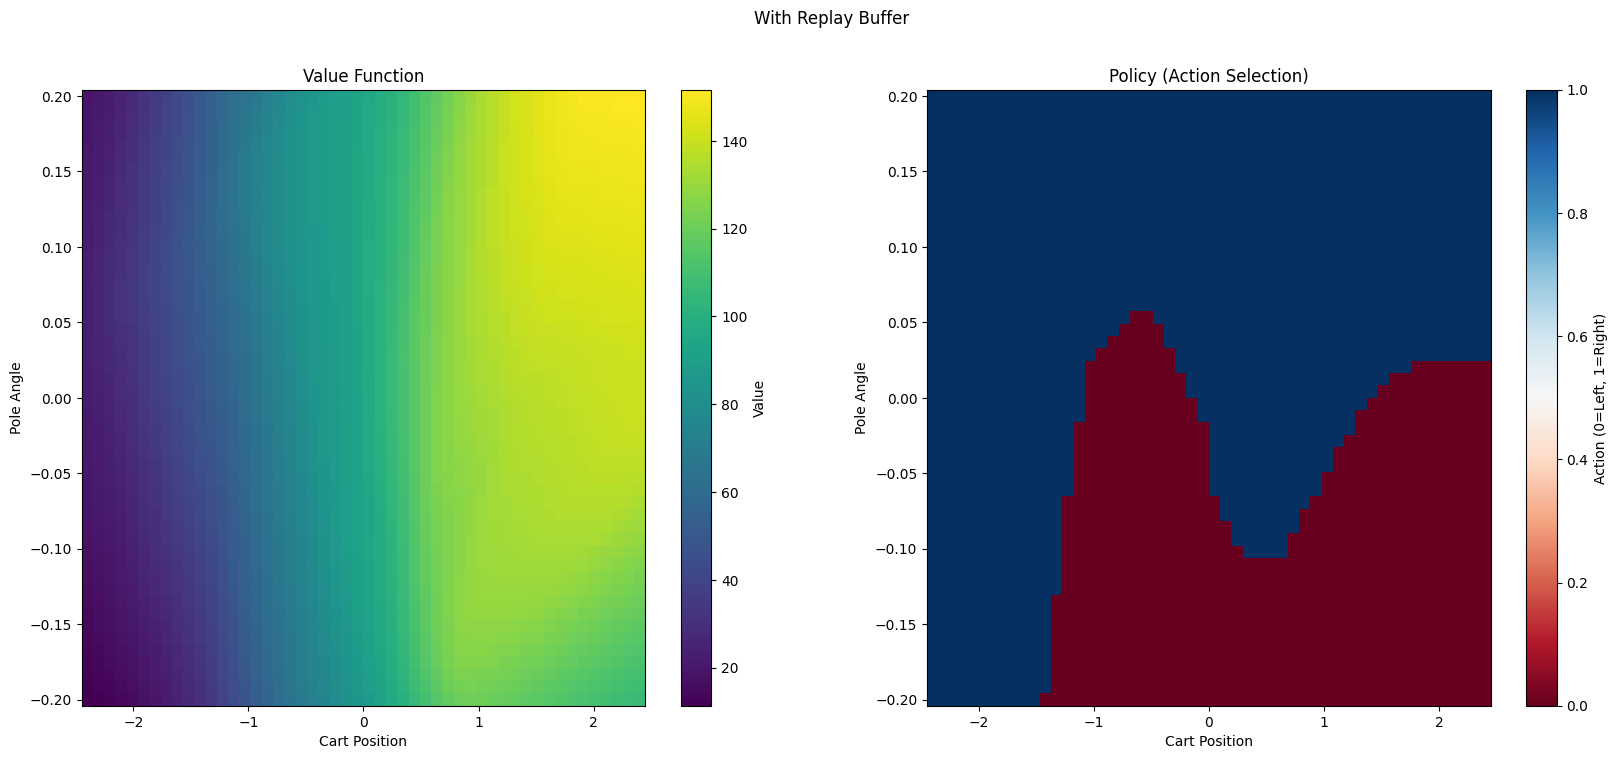
\includegraphics[width=0.9\textwidth]{images/1b_3.png}
		\caption{Value function and Policy with regrads to Pole Angle over Cart Position with Replay Buffer}
		\label{fig:5}
	\end{figure}
	\newpage
	
	\textit{Reflection}: 
	The introduction of function approximation enables the algorithm to do Q-Learning even in situations where the state space is really large or continuous, which poses a lot of problems for tabular solutions. Therefore, the algorithm is able to adapt to more complicated environments. 
	By introducing a decaying epsilon strategy, the algorithm has time to explore the environment before then converging on the learned policy. With function approximation, the algorithm still explores when having explored enough, which leads to problems with stability. 
	This problem can be adressed with a replay buffer, which helps stabilize the resulting Q-Network, since it doesnt learn on correlated data, which is the case when using consecutive samples in a regular DQN
	Also, the introduction of a target network helps to stabilize the learning process, since it reduces the variance of the updates, which can be a big problem for high gammas especially.
	These stability changes can be perceived in the graphs, where the average loss and reward are more stable when using a replay buffer and a target network, and of course the advanced algorithm converges to a almost perfect policy. 
	
	
	
\end{document}